\documentclass[12pt,addpoints,answers]{guia}
\grado{3$^\circ$ de Secundaria}
\cicloescolar{2022-2023}
\materia{Ciencias y Tecnología: Química}
\guia{22}
\unidad{3}
\title{Enlaces químicos}
\aprendizajes{
    \begin{itemize}[leftmargin=*,label=\small\color{colorrds}\faIcon{user-graduate}]
        \item Identifica componentes químicos importantes que participan en la estructura y funciones del cuerpo humano. 
        \item Representa y diferencia elementos y compuestos, así como átomos y moléculas.
        \item Explica y predice propiedades físicas de los materiales con base en modelos submicroscópicos.
    \end{itemize}
}
\author{JC Melchor Pinto}
\begin{document}
\pagestyle{headandfoot}
%\thispagestyle{plain}

\INFO
\printanswers
\begin{multicols}{2}
    \include*{../blocks/block022b}
    \include*{../blocks/block022c}
    \include*{../blocks/block022d}
\end{multicols}
\begin{questions}
    \section{Introducción}
    \vbox{\leftskip\leftmargin Los seres vivos se componen de átomos, pero en la mayoría de los casos, esos átomos no están flotando por ahí individualmente. Por el contrario, generalmente están interactuando con otros átomos (o grupos de átomos).\\

        Como ejemplo, los átomos podrían estar conectados por enlaces fuertes y organizados en moléculas o cristales; o podrían formar enlaces temporales y débiles con otros átomos con los que chocan o rozan. Tanto los enlaces fuertes, que mantienen unidas a las moléculas, como los enlaces más débiles que crean conexiones temporales, son esenciales para la química de nuestros cuerpos y la existencia de la vida misma.\\

        ¿Por qué formar enlaces químicos? La respuesta fundamental es que los átomos están tratando de alcanzar el estado más estable (de menor energía) posible. Muchos átomos se vuelven estables cuando su orbital de valencia está lleno de electrones o cuando satisfacen la regla del octeto (al tener ocho electrones de valencia). Si los átomos no tienen este arreglo, ``desearán'' lograrlo al ganar, perder o compartir electrones mediante los enlaces.}
    \question[99] pregunta 1



    \section{Los iones y los enlaces iónicos}

    Algunos átomos se vuelven más estables al ganar o perder un electrón completo (o varios electrones). Cuando lo hacen, los átomos forman iones, o partículas cargadas. El ganar o perder electrones le puede dar a un átomo una capa electrónica externa llena y hacer que sea energéticamente más estable.

    \subsection{La formación de iones}
    Los iones pueden ser de dos tipos. Los cationes son iones positivos que se forman al perder electrones. Por ejemplo, un átomo de sodio pierde un electrón para convertirse en un catión sodio,Na$^+$.
    Los iones negativos se forman al ganar electrones y se llaman aniones. Los aniones reciben nombres que terminan en "-uro"; por ejemplo, el anión del cloro (Cl$^-$) se llama \emph{cloruro}.
    Cuando un átomo pierde un electrón y otro átomo gana un electrón, el proceso se conoce como transferencia de electrones. Los átomos de sodio y de cloro son un buen ejemplo de transferencia de electrones.
    El sodio (Na) solo tiene un electrón en su capa electrónica externa, por lo que es más fácil (más electrónicamente estable) que el sodio done ese electrón a que encuentre siete electrónes más para llenar su capa externa. Debido a esto, el sodio tiende a perder su único electrón y formar Na$^+$.Por otra parte, el cloro (Cl), tiene siete electrones en su capa externa. En este caso, es más fácil para el cloro ganar un electrón que perder siete, entonces tiende a tomar un electrón y convertirse en Cl$^-$.
    El sodio transfiere uno de sus electrones de valencia al cloro, lo que resulta en la formación de un ion sodio (que no tiene electrones en su tercera capa, lo que significa que su segunda capa está completa) y un ion cloruro (con ocho electrones en su tercera capa, lo que le da un octeto estable).
    Cuando se combinan el sodio y el cloro, el sodio donará su electrón para vaciar su capa más externa, y el cloro aceptará ese electrón para llenar la suya. Ahora ambos iones satisfacen la regla del octeto y tienen capas externas completas. Dado que el número de electrones ya no es igual al número de protones, cada átomo se ha convertido en un ion y tiene una carga +1 (Na$^+$) o -1 (Cl$^-$).

    En general, un átomo debe perder un electrón al mismo tiempo que otro átomo gana un electrón: para que un átomo de sodio pierda un electrón, necesita tener un receptor adecuado como un átomo de cloro.

    \subsection{La formación de un enlace iónico}
    Los enlaces iónicos son enlaces que se forman entre iones con cargas opuestas.
    Por ejemplo, los iones sodio cargados positivamente y los iones cloruro cargados negativamente se atraen entre sí para formar cloruro de sodio o sal de mesa. La sal de mesa, al igual que muchos compuestos iónicos, no se compone solo de un ion sodio y un ion de cloruro; por el contrario, contiene muchos iones acomodados en un patrón tridimensional predecible y repetido (un cristal).
    En la última sección, analizamos cómo el sodio puede perder un electrón para formar el catión Na$^+$, y por otra parte, cómo el cloro puede ganar un electrón para formar el anión Cl$^-$. Pero en realidad este proceso puede ocurrir completo en un solo paso cuando el sodio regala su electrón al cloro. Podemos ilustrar esto como sigue:

    \begin{figure}[H]
        \centering
        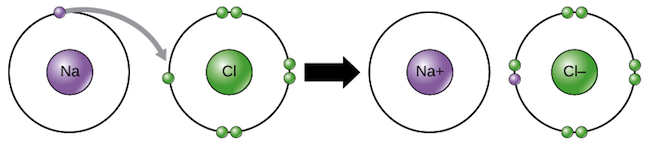
\includegraphics[width=0.8\linewidth]{../images/a05bd453d0dc5add39892ed10f63bc92a5508539}
        \caption{El sodio dona su electrón al cloro para formar Na$^+$ y Cl$^-$. Crédito de la imagen: Boundless Learning (Aprendizaje sin límites), CC BY-SA 4.0}
        \label{fig:enlace_ionico}
    \end{figure}

    Aquí podemos ver cómo se transfiere un electrón del sodio al cloro para formar los iones Na$^+$ y Cl$^-$. Una vez que se forman estos iones, hay una fuerte atracción electrostática entre ellos, lo que lleva a la formación de un enlace iónico. Podemos ver que uno de los principales factores que distingue los enlaces iónicos de los covalentes es que en los enlaces iónicos los electrones se transfieren completamente, mientras que en los enlaces covalentes, los electrones se comparten.

    \begin{importantbox}
        En la fisiología, ciertos iones se conocen como electrolitos (como sodio, potasio y calcio). Estos iones son necesarios para la conducción de impulsos nerviosos, la contracción muscular y el equilibrio de agua. Muchas bebidas deportivas y suplementos dietéticos proporcionan iones para reponer aquellos que se pierden durante el ejercicio por la sudoración.
    \end{importantbox}

    pregunta sobre enlaces ionicos

    \subsection{El dibujo de enlaces iónicos}
    Ahora consideraremos las diferentes maneras de dibujar o representar los enlaces iónicos. Seguiremos estudiando el compuesto iónico más comúnmente conocido, el cloruro de sodio, también llamado sal de mesa. Se puede representar un solo enlace iónico en el cloruro de sodio de la siguiente manera:

    \begin{figure}[H]
        \centering
        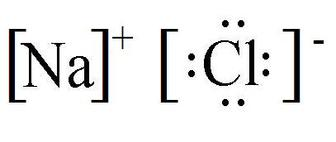
\includegraphics[width=0.8\linewidth]{../images/5ea8232d69862ad00d65c8d625907b7e1b04172e}
        \caption{Diagrama estructural que muestra un enlace iónico entre un catión de sodio, Na$^+$, y un anión de cloruro, Cl$^-$. Observa que no hay una línea que conecte los dos iones porque eso indicaría que comparten electrones en un enlace covalente. Aquí, los electrones se transfirieron completamente, y el enlace es puramente iónico. Crédito de la imagen: Wikispaces, CC BY-SA 3.0}
        \label{fig:5ea8232d69862ad00d65c8d625907b7e1b04172e}
    \end{figure}

    Al catión de sodio con carga positiva y al anión de cloruro con carga negativa les gusta colocarse uno junto al otro debido a su atracción electrostática mutua. Puesto que no se comparten electrones, no mostramos un enlace iónico con una línea como lo hacemos para los enlaces covalentes. Sencillamente reconocemos que la atracción existe por los signos de cargas opuestas en los iones.
    El diagrama anterior, sin embargo, es solo un modelo. En la naturaleza, el cloruro de sodio no existe como un solo catión de sodio unido con un solo anión de cloruro. Como mencionamos antes, el cloruro de sodio es la sal de mesa, y si pudiéramos usar un microscopio superpoderoso con en el que fuera posible ver la sal de mesa a nivel atómico, veríamos algo como la estructura siguiente:

    \begin{figure}[H]
        \centering
        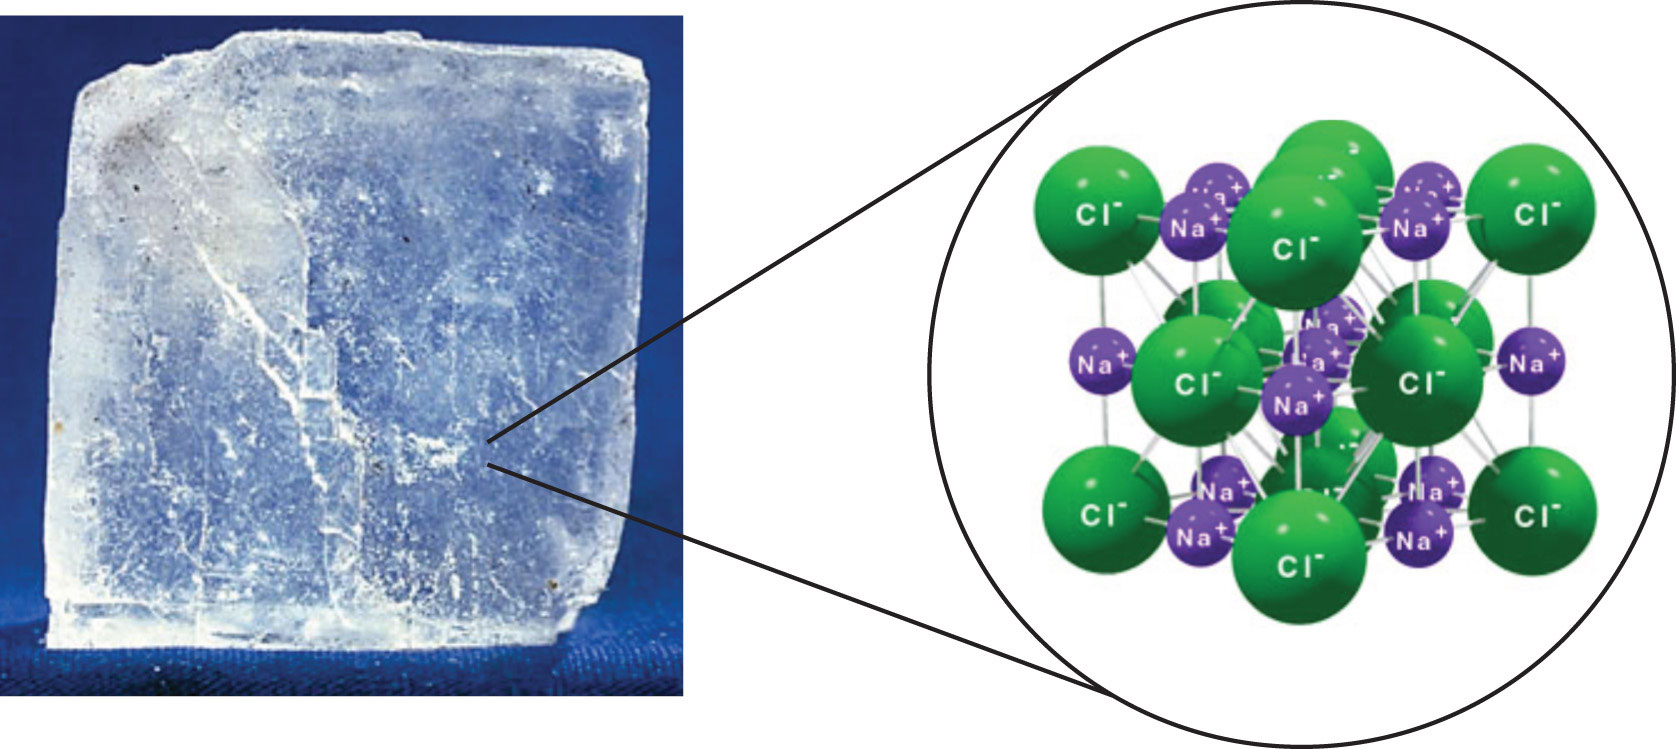
\includegraphics[width=0.8\linewidth]{../images/99e84686a2a3381cdbf8e264a8b94dd1a9c26f41}
        \caption{Si examináramos un cristal de cloruro de sodio a nivel atómico, veríamos los iones de sodio y de cloruro repartidos uniformemente uno junto al otro en el espacio. Esta estructura ordenada y estable, se debe a los fuertes enlaces iónicos entre Na$^+$ y Cl$^-$. Crédito de la imagen: Introduction to Chemistry: General, Organic, and Biological (Introducción a la química: general, orgánica y biológica), CC BY-NC-SA 3.0}
        \label{fig:99e84686a2a3381cdbf8e264a8b94dd1a9c26f41}
    \end{figure}

    En este diagrama podemos ver que los iones Na$^+$ y Cl$^+$ se colocan naturalmente uno junto al otro en el espacio debido a la atracción electrostática que comparten entre ellos. Entonces los iones se mantienen en su lugar mediante sus enlaces iónicos muy fuertes. La estructura anterior se conoce como red cristalina, y el cloruro de sodio, como la mayoría de los compuestos iónicos, es un sólido cristalino. Aprenderás más sobre esto en lecciones futuras sobre los diferentes tipos de sólidos.

    \section{Enlaces covalentes}
    Otra manera como los átomos se vuelven más estables es al compartir electrones (en lugar de ganarlos o perderlos por completo), formando así enlaces covalentes. Estos enlaces son mas comunes que los enlaces iónicos en las moléculas de los organismos vivos.

    Se forma un enlace covalente cuando dos átomos comparten pares de electrones. En un enlace covalente, la estabilidad del enlace proviene de la atracción electrostática que comparten los dos núcleos atómicos con carga positiva, y los electrones con carga negativa que comparten entre los dos.
    20230321200703.png
    \begin{figure}[H]
        \centering
        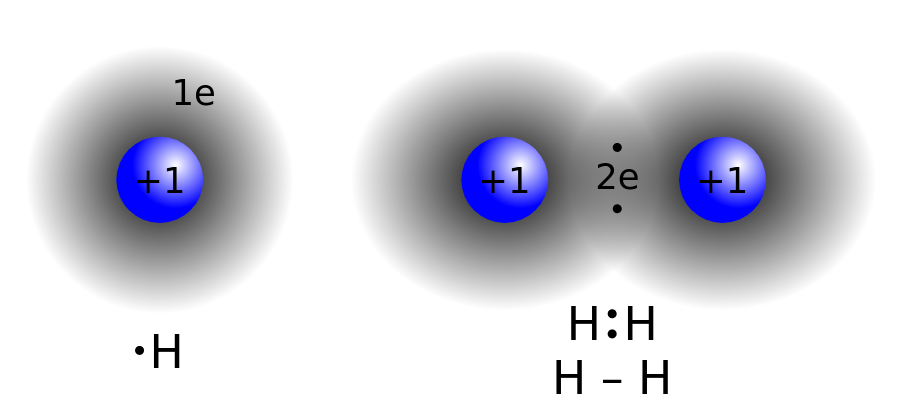
\includegraphics[width=0.8\linewidth]{../images/20230321200703}
        \caption{Un átomo de hidrógeno neutro, a la izquierda, contiene un electrón. Dos átomos de hidrógeno se pueden combinar al donar cada uno de sus electrones a un solo enlace covalente, que se muestra a la derecha como el área donde las nubes grises alrededor de cada hidrógeno se sobreponen. En el enlace covalente, los dos átomos de hidrógeno comparten el par de electrones. Cuando se forma el enlace covalente, ya no tenemos dos átomos de hidrógeno separados, sino una sola molécula de hidrógeno: H$_2$. Crédito de la imagen: Wikipedia, CC BY-SA 3.0}
        \label{fig:20230321200703}
    \end{figure}

    Cuando se combinan los átomos al formar enlaces covalentes, el grupo de átomos que resulta se conoce como molécula. Por lo tanto, podemos decir que una molécula es la unidad más simple de un compuesto covalente. Como ahora podremos ver, hay una variedad de formas distintas de representar y dibujar moléculas.

    Por ejemplo, los enlaces covalentes son clave para la estructura de las moléculas orgánicas basadas en el carbono, como nuestro ADN y proteínas. También hay enlaces covalentes en moléculas inorgánicas más pequeñas, tales como H$_2$O, CO$_2$, y O$_2$. Se pueden compartir uno, dos o tres pares de electrones, lo que resulta en enlaces simples, dobles o triples, respectivamente. Entre más electrones compartan dos átomos, más fuerte será el enlace.
    Como ejemplo de enlace covalente, examinemos el agua. Una sola molécula de agua, H$_2$O, está compuesta de dos átomos de hidrógeno unidos a un átmo de oxígeno. Cada hidrógeno comparte un electrón con el oxígeno y el oxígeno comparte uno de sus electrones con cada hidrógeno:
    Átomos de hidrógeno que comparten electrones con un átomo de oxígeno para formar enlaces covalentes al crear una molécula de agua
    Los electrones compartidos dividen su tiempo entre las capas de valencia de los átomos de hidrógeno y oxígeno, y le dan a cada átomo algo que se parece a una capa de valencia completa (dos electrones para el H, y ocho para el O). Esto hace que una molécula de agua sea mucho más estable de lo que serían los átomos que la componen por sí solos.

    \subsection{Enlaces covalentes polares}
    Hay dos tipos principales de enlaces covalentes: polar y no polar. En un enlace covalente polar, los electrones se comparten de forma no equitativa entre los átomos y pasan más tiempo cerca de un átomo que del otro. Debido a la distribución desigual de electrones entre los átomos de diferentes elementos, aparecen cargas ligeramente positivas ($\delta$+) y ligeramente negativas ($\delta$-) en distintas partes de la molécula.
    En una molécula de agua (arriba), el enlace que une al oxígeno con cada hidrógeno es un enlace polar. El oxígeno es un átomo mucho más electronegativo que el hidrógeno, por lo que el oxígeno del agua tiene una carga parcialmente negativa (tiene una densidad de electrones alta), mientras que los hidrógenos llevan cargas parcialmente positivas (tienen una densidad electrónica baja).
    En general, la electronegatividad relativa de los dos átomos en un enlace, es decir su tendencia a acaparar los electrones compartidos, determinará si el enlace es polar o no polar. Siempre que un elemento sea significativamente más electronegativo que otro, el enlace entre ellos será polar; esto significa que uno de sus extremos tendrá una carga ligeramente positiva y el otro una carga ligeramente negativa.

    \subsection{Enlaces covalentes no polares}
    Los enlaces covalentes no polares se forman entre dos átomos del mismo elemento o entre átomos de diferentes elementos que comparten electrones de manera más o menos equitativa. Por ejemplo, el oxígeno molecular (O$_2$) no es polar porque los electrones se comparten equitativamente entre los dos átomos de oxígeno.
    Otro ejemplo de enlace covalente no polar puede encontrarse en el metano (CH$_4$). El carbono tiene cuatro electrones en su capa exterior y requiere cuatro más para volverse un octeto estable. Los consigue al compartir electrones con cuatro átomos de hidrógeno, cada uno de los cuales le provee de un electrón. Del mismo modo, los átomos de hidrógeno necesitan un electrón adicional cada uno para llenar su capa más externa, los cuales reciben en forma de electrones compartidos del carbono. Aunque el carbono y el hidrógeno no tienen exactamente la misma electronegatividad, son bastante similares, así que los enlaces carbono-hidrógeno se consideran no polares.
    Tabla que muestra al agua y al metano como ejemplos de moléculas con enlaces polares y no polares, respectivamente


    \section{Compuestos covalentes vs compuestos iónicos: moléculas vs celdas unidadarias}
    Ya que hemos analizado lo básico tanto de los enlaces covalentes como de los iónicos, tenemos que hacer unas cuantas diferencias necesarias. Sabemos que un grupo de átomos unidos solo por enlaces covalentes se conoce como molécula. Se debe enfatizar, sin embargo, que la palabra molécula solo se debe usar para referirse a compuestos covalentes. En un compuesto iónico, como el cloruro de sodio, no existe algo como una sola molécula de cloruro de sodio, puesto que en realidad, el cloruro de sodio está hecho de muchos iones de sodio y cloro unidos en una gran red cristalina, como lo vimos en el diagrama anterior. Como tal, nos referimos a un pedazo de NaCl no como una molécula sino como una celda unidadaria. Hay que tener en cuenta que una sola celda unidadaria, a diferencia de una sola molécula, en general no existe en la naturaleza, simplemente usamos las celdas unidadarias por conveniencia y para facilitar su alusión.

    ¿Qué tipo de compuestos están hechos de moléculas, los iónicos o los covalentes?

    \begin{solutionbox}{1.2cm}
        Los compuestos covalentes están hechos de moléculas.
    \end{solutionbox}

    \section{Conclusión}
    Todos los enlaces químicos se deben a la atracción electrostática. Cuando los átomos se combinan a través de enlaces químicos, forman compuestos, es decir estructuras únicas que se conforman de dos o más átomos. La composición básica de un compuesto se puede manifestar mediante el uso de una fórmula química. Una fórmula química utiliza símbolos de la tabla periódica para indicar los tipos de elementos presentes en un compuesto en particular, y usa subíndices para representar el número de cada tipo de elemento presente.
    Los compuestos pueden ser covalentes o iónicos. En los compuestos covalentes, los átomos forman enlaces covalentes que consisten de núcleos atómicos adyacentes que comparten pares de electrones. Un ejemplo de compuesto covalente es el amoniaco. La fórmula química del amoniaco es NH$_3$, que nos dice que en una sola molécula de amoniaco hay un átomo de nitrógeno y tres átomos de hidrógeno. La estructura de un compuesto covalente se puede representar a través de modelos espaciales así como de modelos de esferas y barras.
    En los compuestos iónicos, los electrones se transfieren completamente de un átomo a otro, de manera que se forma un catión (ion con carga positiva), y un anión (ion con carga negativa). La fuerte atracción electrostática entre cationes y aniones adyacentes se conoce como enlace iónico. El ejemplo más común de un compuesto iónico es el cloruro de sodio, NaCl, mejor conocido como sal de mesa. A diferencia de los compuestos covalentes, no existe algo como una molécula de un compuesto iónico. Esto se debe a que en la naturaleza, el NaCl no existe en unidades individuales, sino en estructuras de red cristalina que se conforman de muchos iones de Na$^+$ y Cl$^-$ que se alternan en el espacio. La fórmula química NaCl especifica una celda unidadaria de este compuesto.
\end{questions}
\end{document}
